\chapter{Attitude control}
\section{Modelling}
This section provides a description of the dynamic and kinematic equations of motion which constitute the basis for further analysis and description of the forces and/or disturbances, which may affect a rigid body within LEO. The model for the satellite is derived based on rigid body dynamics and kinematics. 
%In order to control the distance between two or more satellites in orbit, a mathematical description of the governing equations should be derived. Since precious work have been made in previous projects, and all the measurements are available, in-depth analysis it is deemed not necessary. 
%
\subsection{Kinematics}
This section will provide the orbit-attitude determination of the satellite using quaternion representation. 

Quaternion parameterization is deemed useful for the kinematic analysis of the satellite. The orientation of the rigid body at time $t$ is represented as $\vec q(t)$ and at time $\vec q(t+\Delta{t})$ is the resulting quaternion at time $t+\Delta{t}$. The orientation of $\vec q(t+\Delta t)$ can be found by multiplying the quaternion at time $t$ and the rotations of the satellite during the interval $\Delta t$, as follows \cite{SADC}:
%
\begin{flalign}
	\vec{ ^s_iq}(t+\Delta{t}) = \vec{ q}(\Delta {t}) \otimes \vec{ ^s_i q}(t) 
	\label{eq:quaternionproduct}
\end{flalign}
%
The axis $\vec{\hat{x}}, \vec{\hat{y}}, \vec{\hat{z}}$  are the three axis of the satellite body frame at time $t$ and $[e_{x} \ e_{y} \ e_{z}]$ are the components of the rotation axis unit vector along $\vec{\hat{x}}, \vec{\hat{y}}, \vec{\hat{z}}$. Therefore $q (\Delta {t})$ can be expresed as \cite{SADC}:
%
\begin{flalign}
	q_{1}(\Delta {t})  = {e_{x}\sin\frac{\Delta\Phi}{2}}
	\label{eq:controllerquaternion1}
\end{flalign}
%
\begin{flalign}
	q_{2}(\Delta {t}) = {e_{y}\sin\frac{\Delta\Phi}{2}}
	\label{eq:controllerquaternion2}
\end{flalign}
%
\begin{flalign}
	 q_{3} (\Delta {t})= {e_{z}\sin\frac{\Delta\Phi}{2}}
	\label{eq:controllerquaternion3}
\end{flalign}
%
\begin{flalign}
	q_{4}(\Delta {t}) = {\cos\frac{\Delta\Phi}{2}}
	\label{eq:controllerquaternion4}
\end{flalign}
where
$\Delta \Phi$ is the rotation at time $\Delta t$ 

Combining the  \eqref{eq:controllerquaternion1} - \eqref{eq:controllerquaternion4} with \eqref{eq:quaternionproduct}  results \cite{SADC}: 
%
\begin{flalign}
	\vec{ ^s_i q}(t+\Delta{t})
	= 
	\left\{\cos\frac{\Delta\Phi}{2} \underline I_{(4\times4)}+\sin\frac{\Delta\Phi}{2}
	\begin{bmatrix}
		0 &e_{z}&-e_{y}&e_{x} \\
		-e_{z}&0&e_{x}&e_{y}  \\ 
		e_{y}&-e_{x}&0&e_{z} \\
		-e_{x} &e_{y}&-e_{z}&0
	\end{bmatrix} 
\right \} \vec{ ^s_i q}(t)
	\label{eq:quaternionmult}
\end{flalign}  
%
where $\underline I$ is the $4\times4$ identity matrix. Using the small angle approximation for infinitesimal $\Delta(t)$ and denoted $\vec{\omega}$ the instantaneous change in angular velocity it is obtained 
%
 \begin{flalign}
 	\vec{q(t+\Delta{t})} = \left[1 + \frac{1}{2} \underline \Omega \Delta(t)\right]\vec{q(t)}
 	\label{eq:controllerquaternionfinal}
 \end{flalign} 
with $\underline \Omega$ be the skew symmetric matrix as \cite{SADC}:
\begin{flalign}
	\underline \Omega
	= 
	\begin{bmatrix}
		0& \omega_{z}& - \omega_{y}& \omega_{x} \\
		-\omega_{z}& 0&\omega_{x}& \omega_{y}  \\ 
		\omega_{y}& -\omega_{x}&0& \omega_{z} \\
		-\omega_{x}& -\omega_{y}& -\omega_{z}&0
	\end{bmatrix} 
	\label{eq:skewsymmetricmatrixquaternion}
\end{flalign}
%
the angle approximations where taken as $\cos\frac{\Delta\Phi}{2} \simeq 1$ and $\sin\frac{\Delta\Phi}{2}\simeq \frac{1}{2} \omega \Delta(t) $
%
\subsection{Dynamic Model}
In order to describe the behavior of the satellite a dynamic model based on reaction wheels and using Euler's equation of motion has been derived.   
%
Euler's equation of motion describing the rotation of a rigid body relates the time derivative of angular momentum to the applied torques and is given by \cite{SADC}: 
% 
\begin{flalign}
	\vec{ \dot L} = {\vec{N_{mw}}- \vec{\omega} }{\times \vec{L}}
	\label{eq:eulerequation}
\end{flalign}
% 
where $\vec{N_{tot}}$ represents all the external torques caused from the actuator and the disturbances, $\vec{\omega}$ is the angular velocity of the satellite and $\vec{L}$ is the total angular momentum of the satellite including reaction wheels, given by:
%
\begin{flalign}
	{\vec{L}} = {\underline I_{s}}{\vec{\omega}}+{\vec{h_{mw}}}
	\label{eq:angularmomentum}
\end{flalign}
%
where $\vec{h_{mw}}$ is the vector of the angular momentum of the wheels $[h_1 \ h_2 \ h_3]^{T}$ in the satellites coordinate system and $\underline I_{s}$ is the inertia matrix of the satellite.
%
Inserting the  \eqref{eq:angularmomentum} into \eqref{eq:eulerequation} we obtain:
%
\begin{flalign}
	{\frac{d}{dt}(\underline I_{s}\vec {\omega})+\vec{\dot{h}_{mw}}} =\vec{{N_{mw}}-\vec{\omega}}     {\times  ({\underline I_{s}}{\vec{\omega}} +{\vec{h_{mw}}})}
	\label{eq:angularmomentum2}
\end{flalign}
The derivation of equation of motion can be found in the \appref{chap:A}.
%
For the ease of notation, the cross product can be written as matrix operation using the $\underline S()$ notation representing the skew symmetric matrix  given by:
\begin{flalign}
	{\underline S(\vec \omega)}
	= 
	\begin{bmatrix}
		0& -\omega_{3}& \omega_{2} \\
		\omega_{3}& 0&-\omega_{1}  \\ 
		-\omega_{2} & \omega_{1} &0
	\end{bmatrix} 
	\label{eq:skewsymmetricmatrix}
\end{flalign}
 Solving for $\vec{\dot{\omega}}$ the dynamic equation can be written as 
%
\begin{flalign}
	{\vec{\dot{\omega}}}={-\underline I_{s}^{-1}\underline S(\vec \omega)\underline I_{s}\vec \omega-\underline I_{s}^{-1}\underline S(\vec \omega)\vec h_{mw}-\underline I_{s}^{-1}\vec {\dot{h}_{(mw)}}-\underline I_{s}^{-1}\vec {N_{mw}}}
	\label{eq:angularmomentum3}
\end{flalign} 
%
The rate of change of angular momentum $\vec{\dot{h}_{mw}}$ is given by Newton's second law for rotation:
%
\begin{flalign}
	{\vec{ \dot{h}_{mv}}} = \vec {N_{mw}}
	\label{eq:rate of change}
\end{flalign}
%
The total torque from external disturbances can be written as $\vec{N_{dis}}$. Therefore, \eqref{eq:angularmomentum3} becomes:
%
\begin{flalign}
	{\vec{\dot{\omega}}} ={-\underline I_{s}^{-1}\underline S(\vec \omega)\underline I_{s}\vec \omega-\underline I_{s}^{-1}\underline S(\vec \omega)\vec h_{mw}-\underline I_{s}^{-1}\vec N_{mw}+\underline I_{s}^{-1}\vec N_{dis}}
	\label{eq:angularmomentum4}
\end{flalign}
%
which constitute the dynamics of the satellite with three reaction wheels.  
\subsection{Equation of motion} \label{subsec:eom} 
The behaviour of the satellite attitude is described by the dynamic and kinematic equations, which give a non-linear state space representations.
\begin{flalign}
\begin{bmatrix}
	\vec{ ^s_i\dot q(t)} \\
	\vec{\dot \omega{(t)}}
\end{bmatrix} 	
= 
\begin{bmatrix}
	\frac{1}{2} \underline{ \Omega}_{(4\times4)} \vec{ ^s_i q(t)} \\
	{-\underline{I}_{s}^{-1}\underline{S}(\vec{\omega})\underline{I}_{s}\vec{\omega}(t)-\underline{I}_{s}^{-1}\underline{S}(\vec{\omega})\vec{h_{mw}}-\underline{I}_{s}^{-1}\vec{N_{mw}}(t)+\underline{I}_{s}^{-1}\vec{N_{dis}}(t)}
\end{bmatrix} 
	\label{eq:le}
\end{flalign}
where,\\
  $\vec{ ^s_i \dot q(t)} = [q_1 \ q_2 \ q_3 \ q_4]^T$ \\
  $\vec{\dot \omega{(t)}} = [ \omega_1 \ \omega_2 \ \omega_3]^T$ \\
  $\underline{\Omega}(\omega)$ is the $4\times4$ skew symmetric matrix \\
  $\underline{I}_{s}$ is the inertia matrix \\
  $\underline{S}(\omega)$ is the $3\times3$ skew symmetric matrix \\
  $\vec{N_{dis}}(t)$ is the disturbance torque \\
  $\vec{N_{mw}}$ is the torque from momentum wheels \\
  
 %add underline and vec, h_tot -> h_mw; add the equation for dot(h_mw)
\subsection{Linearized equation of motion} \label{subsec:lem} 
The kinematic and dynamic equations are linearized around the operating point for the purpose of designing a linear controller. The quaternion $\vec{q(t)}$ is split in the operating point ($\vec{\bar{q}}$) and the error quaternion ($\vec{\tilde{q}}$) and the angular velocity $\vec{\omega}$ is split in the nominal value $\vec{\tilde{\omega}}$ and the error $\vec{\tilde{\omega}}$.
\begin{flalign}
	&\vec{ ^s_i q} = \vec{^s_i \bar{q}} \otimes \vec{\tilde{q}} \\
	&\vec{\tilde{q}} = \vec{ ^s_i \bar{q}}^{-1} \otimes \vec{^s_i q} \\
	&\vec{\omega} = \vec{\bar{\omega}} + \vec{\tilde{\omega}} 
	\label{eq:smallsignal}
\end{flalign}
	 Thus, the linearized equation of motion for the satellite are given by \cite{TH}: 
\begin{flalign}
	\begin{bmatrix}
		\vec{ \dot {\tilde{q}}(t) } \\
	\vec{ \dot {\tilde{\omega}}(t) }
	\end{bmatrix} 	
	= 
	\begin{bmatrix}
	-\underline{S}(\vec{\bar{\omega}}) &	\frac{1}{2} \underline{\vec 1}_{(3\times3)} \\
	 \underline{ 0}_{(3\times3)} &	{\underline{I}_{s}^{-1}\underline{S}(\underline{I}_{s} \vec \omega(t))-\underline{I}_{s}^{-1}\underline{S}(\vec \omega)\underline{I}_{s}}
	\end{bmatrix} 
		\begin{bmatrix}
		\vec{  {\tilde{q}}(t) } \\
		{  {\tilde{\omega}}(t) }
    	\end{bmatrix} 	
-
	\begin{bmatrix}
	\underline{\vec 0}_{(3\times3)} \\
		{\underline I_{s}^{-1}}
    \end{bmatrix} 	
  \vec {\tilde N_{mw}}
	\label{eq:lele}
\end{flalign}

\section{Disturbance Models}\label{sec:csf} 
\subsection{Gravity-Gradient torque}
An unbalanced satellite in orbit is subjected to a torque due to Earth's non-uniform gravitational field. Assumed that the Earth is a point mass and the satellite is a rigid body, the gravitational torque can be estimated. Each infinitesimal element of the satellite of mass \textit{$dm_i$} is subjected to an infinitesimal force \textit{$\vec dF_i$} acting on the mass element located at position $\vec R{i}$ from the earth's geometric centre that can be calculated as  \cite{SADC}:
\begin{flalign}
d\vec{F_i} = -G\frac{m_{earth}}{\vec R_i^3}dm_i \cdot \vec{R_i}
	\label{eq:ref1}
\end{flalign}
where $G$ is the gravitational constant, $m_{earth}$ is the mass of the earth and $\vec{R_i}$ is the vector from the Earth's geometric centre to the infinitesimal element of the satellite. 

The torque about the geometric centre of the satellite due to a force \textit{$dF_i$} at a distance $r_i$ from the geometric centre of the satellite is calculated as:
\begin{flalign}
	d\vec{N_{gra}} =  \vec r_i \times d\vec{F_i} 
	\label{eq:ref2}
\end{flalign}
 $\vec r_i$ can be written as the sum of two vectors as seen in the \figref{fig:ggt}, $\vec r_{co}$ which is the vector from geometric centre of the satellite to the centre of mass, and $\vec r_{ci}$ which is the vector from the centre of mass to the infinitesimal element.  Therefore, the expression of the gravity gradient torque is obtained by integrating \eqref{eq:ref2} and thus obtaining:
\begin{flalign}
	\vec N_{gra} &= \int_{sat} (\vec r_{co} +\vec r_{ci}) \times d\vec{F_i}  
	\label{eq:ref3}
\end{flalign}
\begin{figure}[H]
	\centering
	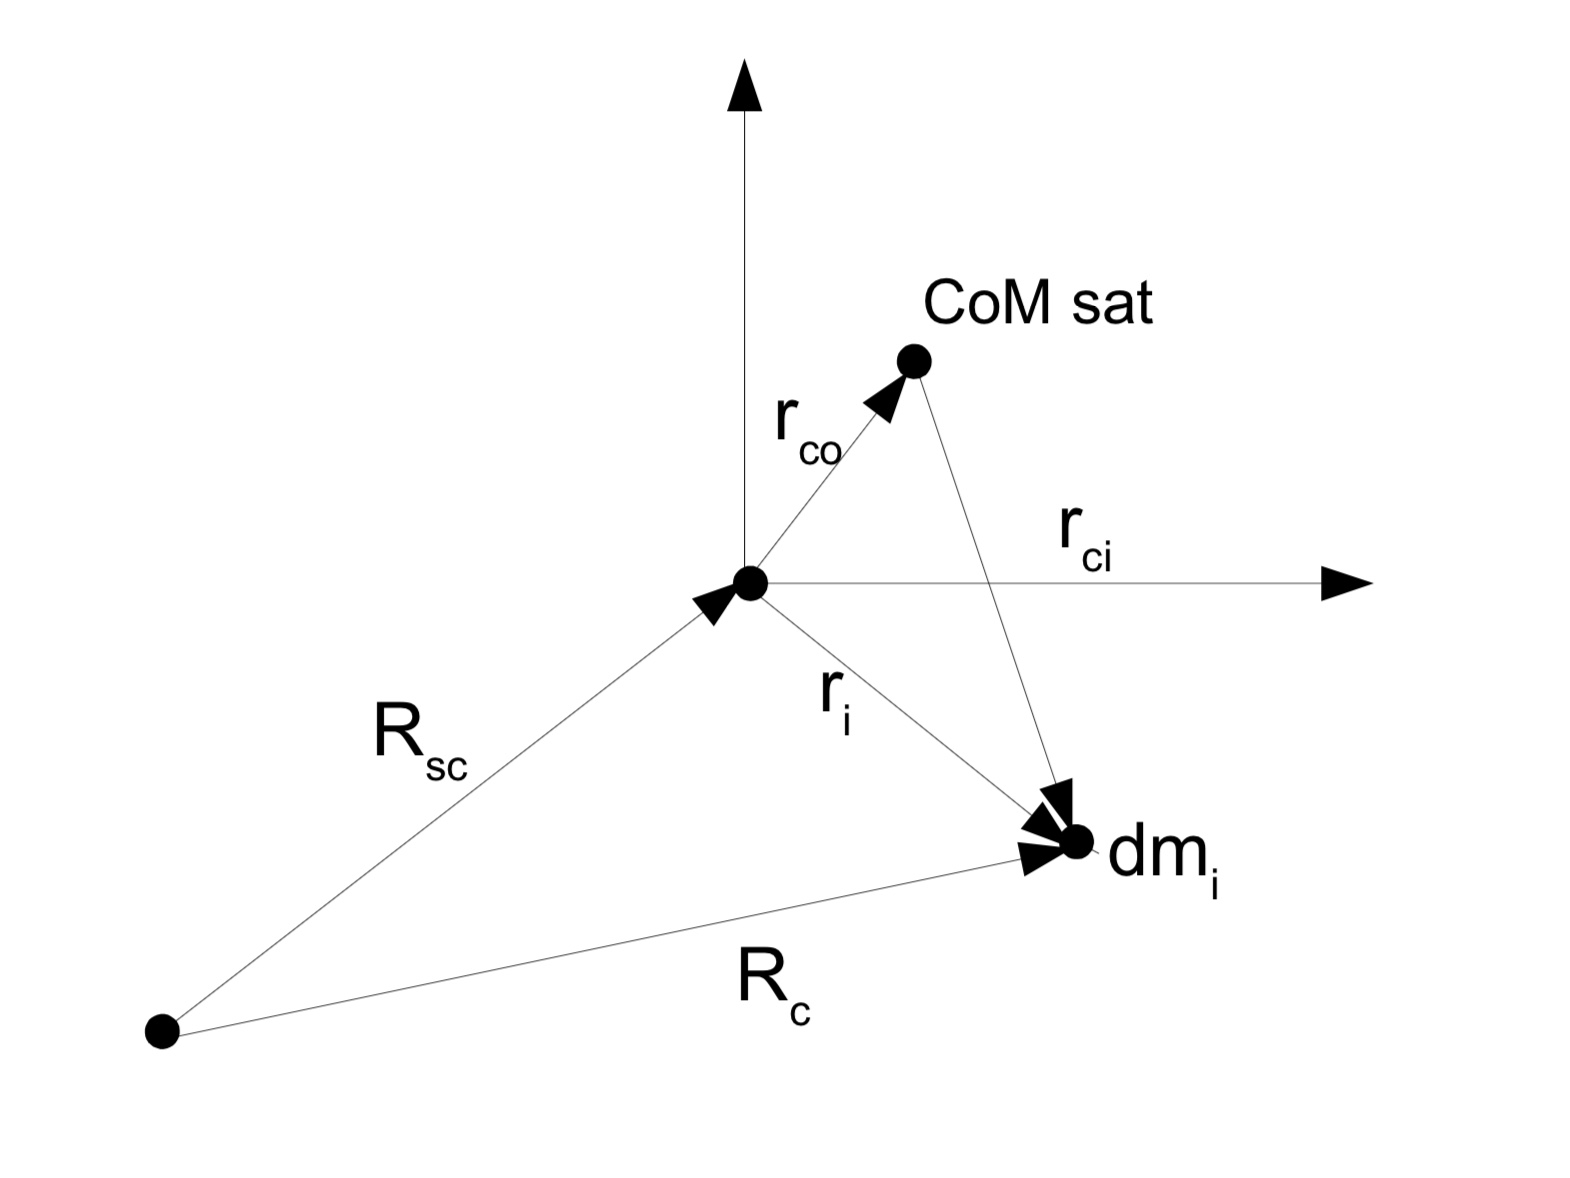
\includegraphics[width=0.6\linewidth]{figures/ggt}
	\caption{Coordinate system for the calculation of gravity gradient torque  \cite{SADC} }
	\label{fig:ggt}
\end{figure}
The vector $\vec{R_i}$ can be written as $\vec{R_i} = \vec{R_{sc}} + \vec{r_i}$. Finally assuming that the geometric centre of the satellite is aligned with its centre of mass, this is equal by setting $r_{co} = 0$, and by using the formula of inertia, and replacing the term $dF_i$ by \eqref{eq:ref1}  the gravity gradient torque can be written as 
%
\begin{flalign}
\vec N_{gra} &= \dfrac{3\mu}{\vec R_{sc}^3}[\vec{\hat R_{sc}} \times(\vec{I} \ \vec{\hat R_{sc}}] 
\label{eq:ref4}
\end{flalign}
where $\vec{\hat R_{sc}}$ is the unit vector from the earth's geometric center to the satellite's geometric center, and $\underline I$ is the diagonal inertia matrix of the satellite. 
\subsection{Solar radiation}
The surface of the CubeSat will absorb or reflect the solar radiation, nevertheless, these two situations will alter the CubeSat, which will produce a torque about the satellite centre of mass (CoM). 
The torque around CoM is given by \cite{SADC}:
\begin{flalign}
	\vec N_{rad} = \vec{F_{rad}} \times \vec R_{CoM}
	\label{eq:tor}
\end{flalign}
where $ \vec F_{rad}$  is the solar radiation  and $\vec R_{CoM}$ is the vector from the centre of mass to the geometric centre of radiation

The solar radiation $\vec F_{rad}$ can be expressed as:
\begin{flalign}
	 \vec F_{rad} = C_{a} P A \ \vec{ \hat{R}_{sun,sat}}
	\label{eq:Pres}
\end{flalign}
where $\vec{ \hat{R}_{sun,sat}}$ is the unit vector with the direction from the sun to the satellite, $C_{a}$ is the surface’s reflectance: 0 for a perfect absorber, 1 for a perfect reflector,   while $P$ is the solar flux and  $A$ is the radiated area

The solar flux can be computed as follows \cite{SADC}:
\begin{flalign}
	P = \dfrac{F_s}{c}
	\label{eq:flux}
\end{flalign}
where $F_s$ is the mean solar energy and it is equal with 1358 $W/m^2$ and $c$ is the speed of light
\subsection{Atmospheric drag}
For objects in LEO, friction with molecules can have a significant impact on the satellite surface by creating a force which acts upon the satellite surface. [ref: sat orbits and missions]. 

The equation of the atmospheric drag force is already computed as shown in \eqref{eq:ec1c}.
Since the force has been computed also the torque can be computed by using the cross product between the drag force and the vector from the center of mass to the center of pressure of the satellite.

The aerodynamic torque acting on the satellite can be written as \cite{SADC}:
\begin{flalign}
	\vec N_{drag} = \vec F_{D} \times \vec r_{s}
	\label{eq:drag}
\end{flalign}
where:\\
$\vec r_{s}$ is the vector from the center of mass to the center of pressure, where the center of pressure is equal with the geometric center of the exposed area\\
$\vec F_D$  is the atmospheric drag force
\section{Attitude control design}
\subsection{Relationship between drag force and quaternion}
In order to apply the desired drag force, a function have to be found to compute the asociated quaternion. A method to find a bijective function between drag force and quaternion is to find two quaternions that give the minimum and the maximum drag force and analyse the drag force in the path between them. 

A quaternion can be defined as a sequence of three rotations around the three axis.
\begin{flalign}
	\vec q = \vec q_x \otimes \vec q_y \otimes \vec q_z
\end{flalign}
with
\begin{flalign}
	\vec q_x = sin \Big(\frac{\theta_x}{2}\Big)*i + cos\Big(\frac{\theta_x}{2}\Big) \\
	\vec q_y = sin \Big(\frac{\theta_y}{2}\Big)*j + cos\Big(\frac{\theta_y}{2}\Big) \\
	\vec q_z = sin \Big(\frac{\theta_z}{2}\Big)*k + cos\Big(\frac{\theta_z}{2}\Big)
\end{flalign}
The drag force can be computed as the folowing:
\begin{flalign}
	u = \frac{u_{min}}{A_{min}}A_{\perp}(\vec{ ^s_o q}) \\
	u = u_{min} \ f(\vec{ ^s_o q} )
\end{flalign}
where $A_{\perp}(\vec{ ^s_o q})$ is the perpendicular area of the satellite with a rotation $\vec{ ^s_o q}$ and $f(\vec{ ^s_o q})$ is defined by $f = \frac{A_{\perp}}{A_{min}}$. Due to the fact that the velocity of the satellite is along the $x$ axis in the orbit frame, a rotation around this axis doesn't change $A_{\perp}$. Therefore, $f$ can be analysed using only rotation around $y$ and $z$ axes. The graph of $f$ in function of $\theta_z$ and $\theta_y$ can be seen in the \figref{fig:perp_area}.
\begin{figure}[H]
	\centering
	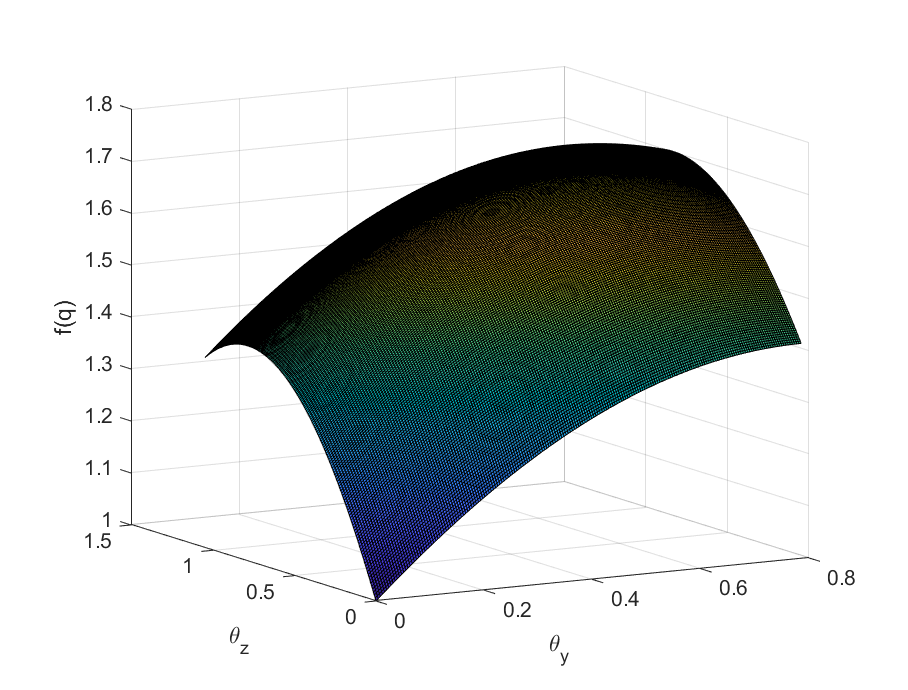
\includegraphics[width= 0.8\linewidth]{figures/perp_area.eps}
	\caption{Perpendicular area in function of rotations around $y$ and $z$ axes}
	\label{fig:perp_area}
\end{figure} 
The quaternion for the minimum drag force is defined by the rotations $\theta_{y,min} = \theta_{z,min} = 0$ and the quaternion that give the maximum drag force is defined by the rotations $\theta_{y,max} = 0.61568$ rad and $\theta_{z,max} = \frac{\pi}{4}$. 

The function $f(\vec{ ^s_o q})$ is computed in the pathm between the minimum and maximum drag force:
\begin{flalign}
	\vec{ ^s_o q} = \vec{ ^s_o q_y} \otimes \vec{ ^s_o q_z} \\
\end{flalign}
with
\begin{flalign}
	\theta_y = \alpha \ \theta_{y,max} \\
	\theta_z = \alpha \ \theta_{z,max}
\end{flalign}
and $ \alpha \in [0,1]$. 

The \figref{fig:path_alpha} shows $f(\vec{ ^s_o q})$ as a function of $\alpha$:
\begin{figure}[H]
	\centering
	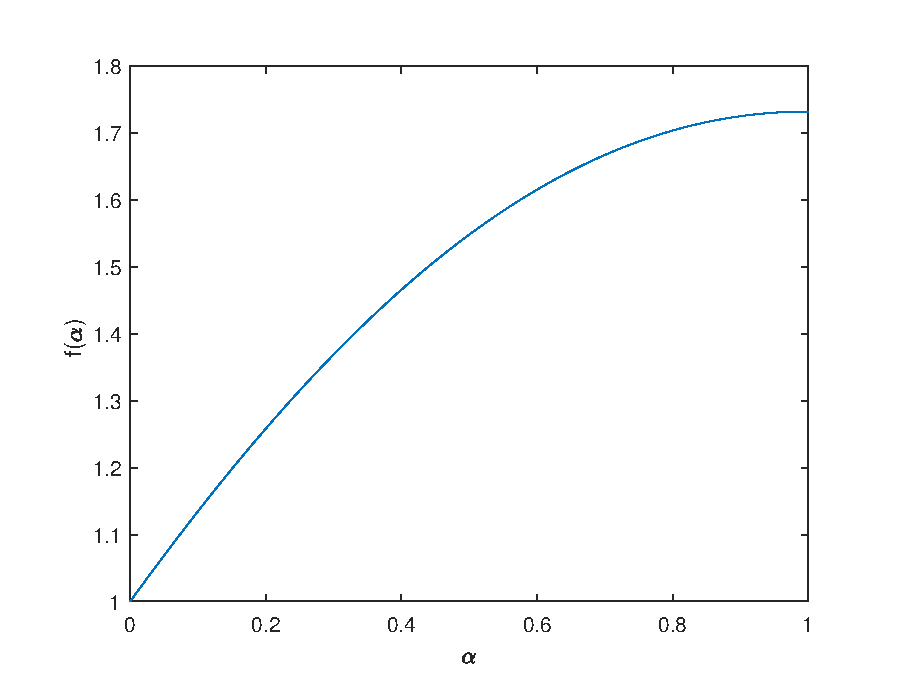
\includegraphics[width=1\linewidth]{figures/path_f.eps}
	\caption{Perpendicular area in function of rotations around $y$ and $z$ axes}
	\label{fig:path_alpha}
\end{figure} 
This function can be approximated by a polynomial of degree two. The relative error of this approximation represented in the \figref{fig:rel_err} is small and thus, the approximation by a polynomial of degree two can be used. 
\begin{figure}[H]
	\centering
	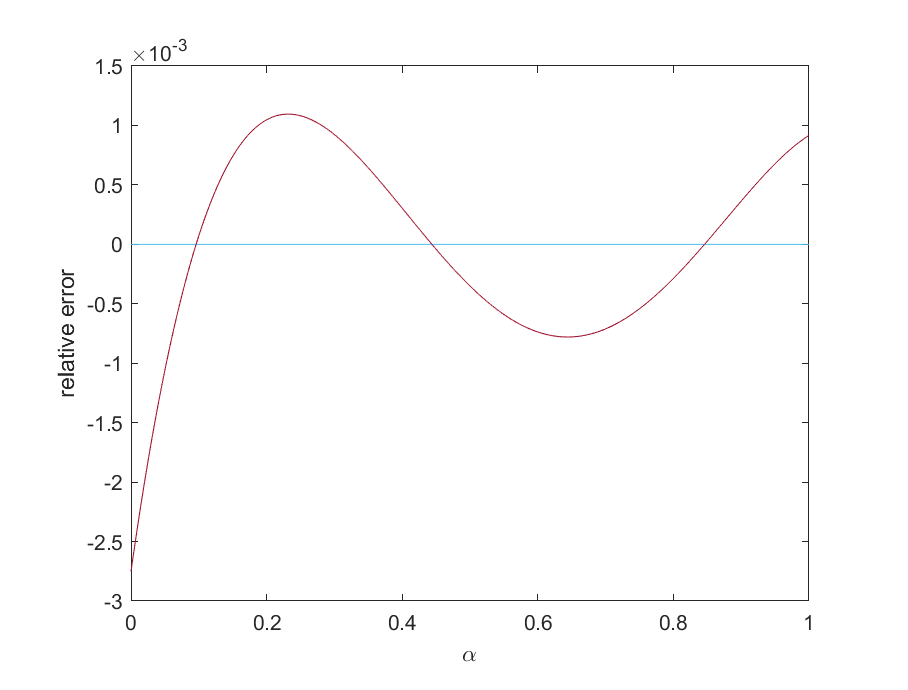
\includegraphics[width=1\linewidth]{figures/rel_err.eps}
	\caption{Relative error of the fitting approximation }
	\label{fig:rel_err}
\end{figure}
Therefore, the quaternion that give the desired drag force in the orbit frame can be computed by following this algorithm:
\begin{flalign}
	\frac{u}{u_{min}} &= f( \alpha ) \approx p_1 \alpha^2 + p_2 \alpha + p_3 \\
	\Rightarrow \alpha &= \frac{-p_2 + \sqrt{p_2^2 - 4 p_1 \Big(p_3 - \dfrac{u}{u_{min}}\Big)}}{2 p_1} \\
	\Rightarrow \theta_y &= \alpha \theta_{y,max} \\
	\theta_z &= \alpha \theta_{z,max} \\
	\Rightarrow \vec{ ^s_o q_y} &= sin\Big(\frac{\theta_y}{2}\Big)*j + cos\Big(\frac{\theta_y}{2}\Big) \\
	\vec{ ^s_o q} &= sin\Big(\frac{\theta_z}{2})*k + cos\Big(\frac{\theta_z}{2}\Big) \\
	\Rightarrow \vec{ ^s_o q_{ref}} &= \vec{ ^s_o q_y} \otimes \vec{ ^s_o q_z}
\end{flalign}
\paragraph{Nota Bene:}
This is one solution of the problem, but there is an infinity of quaternions for one drag force. A better solution would be to choose the reference quaternion that give the desired drag force and that requires the smallest rotation relative to the current position of the satellite. However, this solution is very hard to implemented.
\subsection{Linear Control Design - State Feedback }
The linearized equation \eqref{eq:lele} of the attitude system allows to design a state feedback control. However, the nominal values of the quaternion and the angular velocity depends of the drag force desired and thus, they aren't constant all over the time. Therefore, the designed control have to stabilize the system for all the possibilities of $\bar{q}$ and $\bar{\omega}$. \\

The norm of $\bar{\vec \omega}$ is known and is equal to the angular velocity of the satellite around the Earth ($||\vec{\bar{\omega}}|| \approx 0.0011$). Due to the fact that this value is small compare to $\frac{1}{2}$, the $A$ matrix can be approximated by:

\begin{flalign}
\underline{A}
\approx
\begin{bmatrix}
\underline{0}_{(3\times3)} & \frac{1}{2} \underline{1}_{(3\times3)} \\ \underline{0}_{(3\times3)} & \underline{0}_{(3\times3)}
\end{bmatrix} 
\label{eq:state_feedback}
\end{flalign} 
The system can be split in three subsystems defined by the matrix equation:

\begin{flalign}
\begin{bmatrix}
{ \dot {\tilde{q}}_i}(t)  \\
 {\dot {\tilde{\omega}}_i}(t)
\end{bmatrix} 	
= 
\begin{bmatrix}
0 &	\frac{1}{2}  \\
0 & 0	
\end{bmatrix} 
\begin{bmatrix}
  {{\tilde{q}}}_i(t)  \\
 {{\tilde{\omega}}}_i(t)
\end{bmatrix} 	
+
\begin{bmatrix}
0 \\
{ {I_{i,s}^{-1}}}
\end{bmatrix} 	
{N_{i,c}}(t)
\label{eq:le_bis}
\end{flalign}
where $i$ is equal to 1, 2, 3

The input control torque is defined by a state feedback law:
\begin{flalign}
{N_{i,{mw}}} = 
-\begin{bmatrix}
k_1 & k_2
\end{bmatrix} 
\begin{bmatrix}
{  {\tilde{q}}_i(t) } \\
{{\tilde{\omega}}_i}(t)
\end{bmatrix}
\end{flalign} 
Therefore, 
\begin{flalign}
\underline{A}-\underline{B}\underline{K} = 
\begin{bmatrix}
0 & \frac{1}{2} \\
-\frac{k_1}{I_{i,s}} & -\frac{k_2}{I_{i,s}}
\end{bmatrix}
\end{flalign}
\subsubsection{Pole Placement}
\begin{flalign}
det(s\underline{I}-(\underline{A}-\underline{B}\underline{K})) = s^2 + \frac{k_2}{I_{i,s}} s + \frac{k_1}{2I_{i,s}}
\end{flalign} 
By identification with a general second order equation $s^2 + 2\zeta \omega_n s + \omega_n^2$ where $\zeta$ is the damping factor and $\omega_n$ is the natural frequency, the gains are given by:
\begin{flalign}
k_1 &= -2 \ I_{i,s} \ \omega_n^2 \\
k_2 &= -2 \ I_{i,s} \ \zeta \ \omega_n
\end{flalign}
The damping factor is chosen to be equal to 1 and the rise time is chosen to be equal to 60 and thus $\omega_n = \frac{2\pi}{T_n} = \frac{2\pi}{60/0.35}$. Therefore, all the eigenvalues are equal to -0.0367.
\subsection{Stability}
The stability of control designed in the previous section have to be checked for all $\vec{\bar{\omega}}$. Due to the fact that the matrix A is affine in $\vec{\bar{\omega}}$. The stability can be only checked on the vertices of the convex polyhedron (cube) that contains all the possibilities of $\vec{\bar{\omega}}$ as represented in the \figref{fig:sta_PID}. \cite{NLCS}
\begin{figure}[H]
	\centering
	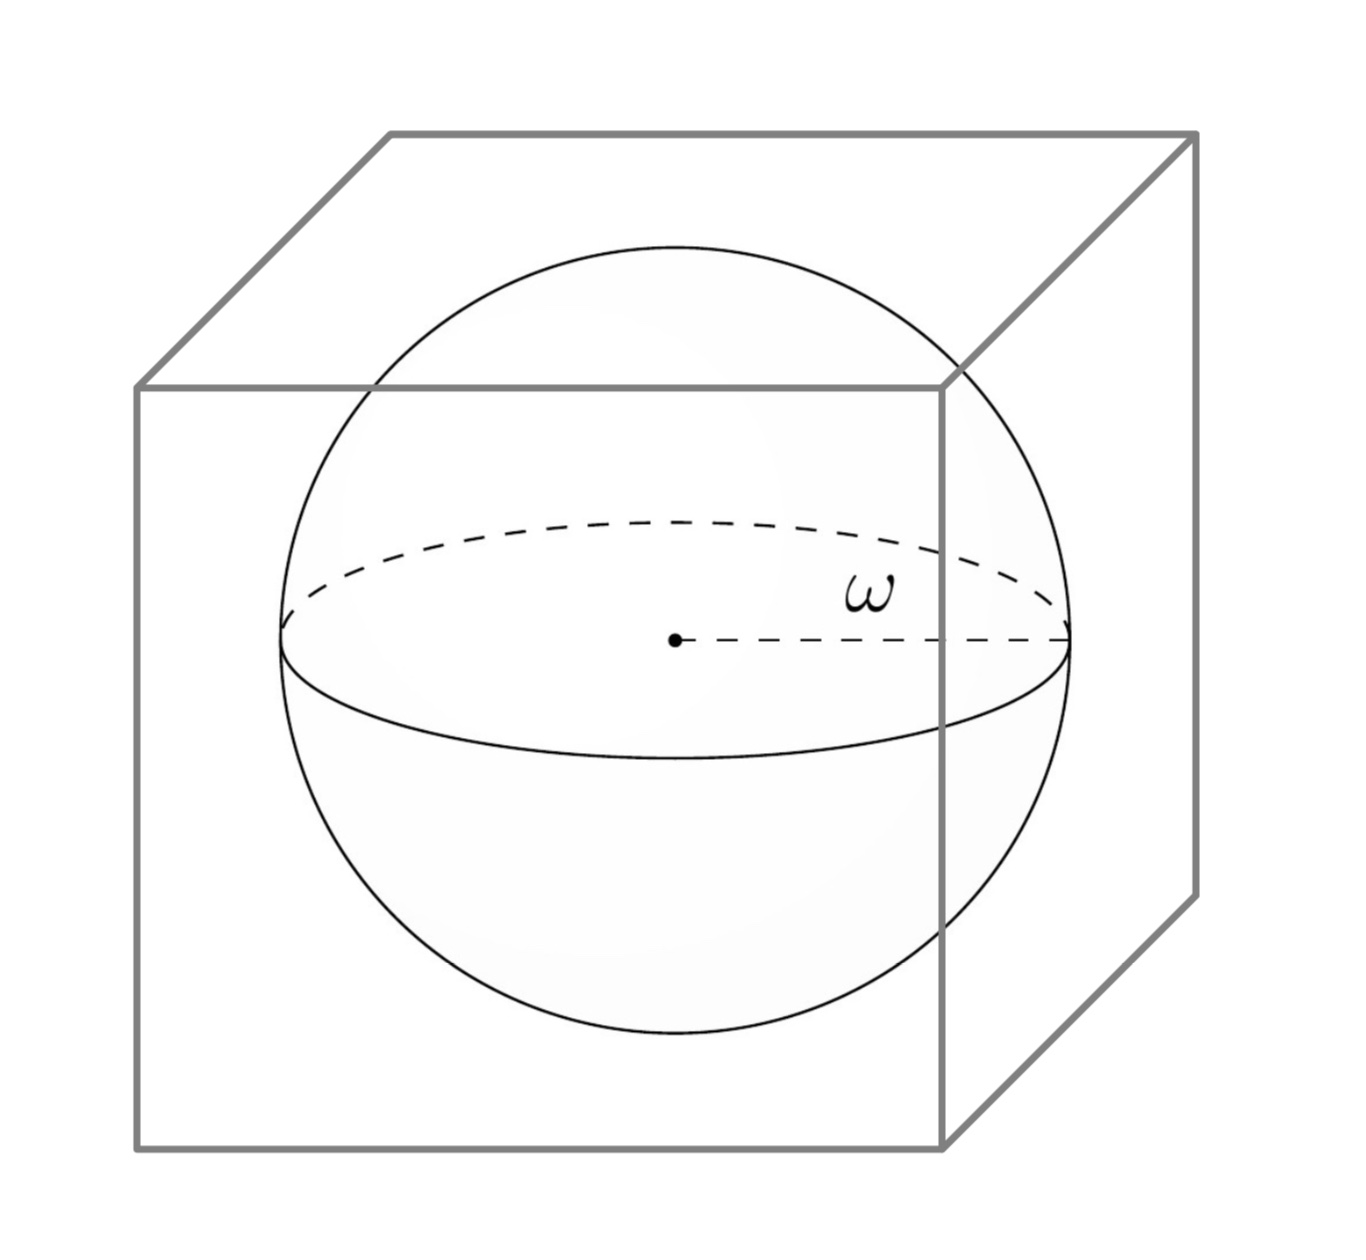
\includegraphics[width=0.4\linewidth]{figures/cs}
	\caption{Convex Polyhedron}
	\label{fig:sta_PID}
\end{figure} 
The maximum real part of the eigenvalue in the vertices of the cube is equal -0.0308 that is very close to the desired eigenvalue.
%
\subsection{Non linear Control Design - Sliding Mode Control }
In parallel to the linear feedback control design also a non-linear method has been designed.A sliding mode controller is implemented in order to compare the differences between the two methods.
%
The sliding mode controller brings the system states to a designed manifold or a hyperplane $s$, such that when the states are on the manifold to converge to the desired reference. If the states are not on the manifold a control law that drives the states to the manifold is necessary. The outcome of this control law is the desired torque that will be fed back to the satellite. The satellite motion can be represented to the space of the sliding variable $s$.
%
The sliding variable can be written in terms of the signal deviation as derived in \eqref{eq:smallsignal}.The quaternion error can be written as \cite{WR}:
\begin{flalign}
	 \vec{\tilde{q}} = \vec{\bar{q}}^{-1} \otimes \vec{q} 
	 =
	\begin{bmatrix}
		q_{4r} & q_{3r}& -q_{2r}& q_{1r}\\
		-q_{3r} & q_{4r}& q_{1r}& q_{2r}\\
		q_{2r} & -q_{1r}& q_{4r}& q_{3r}\\
		-q_{1r} & -q_{2r}& -q_{3r}& q_{4r}\\
	\end{bmatrix} 	
	\begin{bmatrix}
	q_{1} \\ q_{2}\\ q_{3}\\ q_{4}
	\end{bmatrix}
	\label{eq:quat}
\end{flalign}
%
where $\vec{\bar{q}}$ represents the quaternion reference and $\vec{q}$ the measured quaternion. The time derivative of the error quaternion is given by[master thesis]:
\begin{flalign}
\vec{\dot{\tilde{q}}} = \frac{1}{2}\Big(-\vec{q_{\bar{\omega}}} \otimes \vec{\tilde{q}} + \vec{\tilde{q}} \otimes \vec{q_{\bar{\omega}}} + \vec{\tilde{q}} \otimes \vec{q_{\tilde{\omega}}} \Big)
\label{eq:time_deri}
\end{flalign}
%

where $\vec{q_{\bar{\omega}}} = \bar{\omega_{1}}*i +  \bar{\omega_{2}}*j + \bar{\omega_{3}}*k + 0$ and $\vec{q_{\tilde{\omega}}} = \tilde{\omega_{1}}*i +  \tilde{\omega_{2}}*j + \tilde{\omega_{3}}*k + 0$. By choosing the sliding manifold variable to be equal:  
 \begin{flalign}
 	s = F\vec{\tilde{q}} +\vec{\tilde{\omega}}
 	\label{eq:slidingvar}
 \end{flalign}
where $F = d*diag[1 \ 1  \ 1]$ is positive definite. The angular velocity error can be written as $\vec{\tilde{\omega}} = \vec{\omega}  -\vec{\bar{\omega}} $. Therefore, when s = $\vec{0}$, $\vec{ \tilde{\omega} } = -d*\vec{ \tilde{q}_{1:3}}$ and thus the time derivative of the real part of the error quaternion is computed from the equation \ref{eq:time_deri}:
\begin{flalign}
	\dot{\tilde{q}}_{4} &= -\frac{1}{2} \vec{\tilde{\omega}} \cdot \vec{  \tilde{q}_{1:3}} \\
	&= \frac{d}{2}||\vec{\tilde{q}}_{1:3}||^2 \\
	&= \frac{d}{2} \Big(1 - \tilde{q}_4^2\Big)
	\label{eq:dq_4}
\end{flalign} 
According to equation \ref{eq:dq_4}, $\vec{\tilde{q}}$ will converge to $[0; 0; 0; 1]$ and $d$ can be designed by trial and error to have the desired convergence. The behaviour of $\tilde{q}_4$ with $d$ equal to 0.035 is represented in the \figref{fig:dq4}. 
\begin{figure}[H]
	\centering
	\includegraphics[width=0.7\linewidth]{figures/design_D}
	\caption{$\tilde{q}_4$ in function of time with d = 0.035}
	\label{fig:dq4}
\end{figure}  
Assuming a lyapunov candidate function as
\begin{flalign}
	V = \frac{1}{2}s^{T}s
	\label{eq:lyap}
\end{flalign}
the time derivative of the lyapunov fuction can be written as
\begin{flalign}
	\dot V = \frac{1}{2}\Big(\dot{s^{T}}s+s^{T}\dot{s}\Big)
	\label{eq:lyap1}
\end{flalign}
In order to prove stability it has to be shown that $\dot {V} <0 $ $\forall s\neq0$ this is equal by showing 
\begin{flalign}
	 s^{T}\dot{s} < 0 \ \forall s\neq0 
	\label{eq:lyap2}
\end{flalign} 
%
the \eqref{eq:slidingvar} is substitute 
%
\begin{flalign}
	\dot V = s^{T}(F\vec{\dot{\tilde{q}}} +\vec{\dot{\tilde{\omega}}}) 
	\label{eq:lyap3}
\end{flalign}
and using the \eqref{eq:le} for $\vec{\dot{\tilde{\omega}}}$ the \eqref{eq:lyap3} becomes
%
\begin{flalign}
	\dot V = s^{T}\underline I_{s}^{-1}(-{\underline S(\vec \omega)\underline I_{s}\vec \omega-\underline S(\vec \omega)\vec {h_{mw}}-\vec {N_{mw}}+\vec N_{dis}}-I_{s}\dot{\bar{\omega}}+I_{s}F\vec{\dot{\tilde{q}}})
	\label{eq:lyap4}
\end{flalign}
%
where $\bar{\omega}$ is the desired angular velocity. Choosing o control law as
%
\begin{flalign}
	\vec{ N_{mw}} = -\underline S(\vec \omega)\underline I_{s}\vec \omega-\underline S(\vec \omega)\vec h_{mw}-\underline I_s\dot{\omega}+I_{s}F\vec{\dot{\tilde{q}}} +I_{s}{\lambda sign(s)}
	\label{eq:controllaw}
	\end{flalign}
%
the \eqref{eq:lyap4} is written as
%
\begin{flalign}
	\dot V = -s^{T}\underline (-\dot{\tilde{\omega}} + \lambda sign(s) - \vec{N}_{dis}) 
	\label{eq:lyap5}
\end{flalign}
%

Choosing $\lambda > ||\dot{\tilde{\omega}}_{max}|| + ||\vec{N}_{dis}|| $, the condition $\dot {V} <0 $ is satisfied.
\subsubsection{ Sliding Mode Control- simulation}